\section{Esercizio 5 -- Cronometro}
\subsection{Esercizio 5.1}
L'approccio migliore per affrontare la complessità del cronometro è utilizzare un'architettura modulare. Invece di trattare il cronometro come un'unica entità complessa, suddivideremo il problema in parti più gestibili. Ciascuna unità temporale (secondi, minuti e ore) sarà gestita da un contatore separato, rendendo il sistema più modulare e flessibile.

\subsubsection{Implementazione}
\begin{code}
    \inputminted{vhdl}{vhdl/chronometer.vhd}
    \caption{Implementazione del cronometro}
    \label{cod:chronometer}
\end{code}

Il cronometro è stato progettato con un'architettura \texttt{structural} [Codice sorgente \ref{cod:chronometer}], ovvero basata sulla connessione di più componenti, in particolare contatori e un divisore di clock [Figura \ref{fig:5_1_CHRONOMETER}].

\begin{figure}[h]
    \centering
    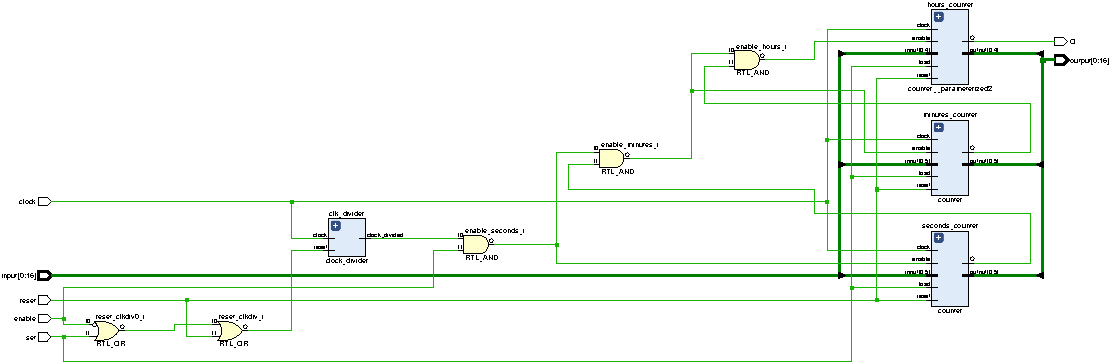
\includegraphics[width=\textwidth]{img/5_1_CHRONOMETER.pdf}
    \caption{Schema a blocchi del cronometro}
    \label{fig:5_1_CHRONOMETER}
\end{figure}

L'obiettivo è scandire il tempo in secondi, minuti e ore utilizzando un segnale di clock di sistema e implementare funzionalità di reset e set per inizializzare il cronometro con un valore predefinito.

\paragraph{Dichiarazione dell’entità.}
L'entità \texttt{chronometer} ha i seguenti ingressi:

\begin{itemize}
    \item \texttt{clock}: segnale di clock principale.
    \item \texttt{enable}: abilita il conteggio del cronometro.
    \item \texttt{reset}: azzera il conteggio.
    \item \texttt{set}: permette di caricare un valore iniziale di ore, minuti e secondi.
    \item \texttt{input}: valore iniziale di ore, minuti e secondi (17 bit totali, suddivisi in 5 bit per le ore, 6 bit per i minuti e 6 bit per i secondi).
\end{itemize}

Inoltre, l'entità ha i seguenti segnali di uscita:

\begin{itemize}
    \item \texttt{output}: valore attuale del cronometro (17 bit come input).
    \item \texttt{Q}: segnale che indica il raggiungimento del massimo valore nel contatore.
\end{itemize}

\paragraph{Componenti utilizzati.}
L'architettura è strutturata utilizzando due tipologie di componenti:

\begin{itemize}
    \item \texttt{clock\_divider} [Codice sorgente \ref{cod:clock_divider}]: il clock di sistema è molto veloce (nel caso della Nexys-7, la frequenza del clock è 100 MHz). Per far avanzare il cronometro di un secondo alla volta, si usa un divisore di clock, che genera un impulso ogni secondo, riducendo la frequenza del clock fino a 1 Hz, in modo che i contatori incrementino solo una volta al secondo.
    \item \texttt{counter} [Codice sorgente \ref{cod:counter_fallingedge}]: tre istanze di contatore con Q sul fronte di discesa vengono utilizzate per contare secondi, minuti e ore  Ogni contatore è dotato di:
    \begin{itemize}
        \item Un massimo di conteggio (\texttt{max\_count}) oltre il quale il conteggio si azzera e viene generato un segnale di overflow (\texttt{Q}).
        \item Ingressi di controllo (\texttt{clock}, \texttt{enable}, \texttt{reset}, \texttt{load}).
        \item Un valore di input per inizializzare il contatore tramite \texttt{set}.
    \end{itemize}
\end{itemize}

\paragraph{Struttura dei tre contatori.}
I contatori sono organizzati in parallelo, così da permettere al segnale di overflow di propagarsi rapidamente tra i contatori. L'organizzazziione è la seguente:

\begin{enumerate}
    \item \texttt{seconds\_counter}: conta fino a 60 (secondi).
    \begin{itemize}
        \item Se arriva a 59 $\rightarrow$ si azzera e genera un segnale \texttt{Q\_seconds} per incrementare i minuti, attivando l’abilitazione \texttt{enable\_minutes}.
    \end{itemize}
    \item \texttt{minutes\_counter}: conta fino a 60 (minuti).
    \begin{itemize}
        \item Se arriva a 59 $\rightarrow$ si azzera e genera un segnale \texttt{Q\_minutes} per incrementare le ore, attivando l’abilitazione \texttt{enable\_hours}.
    \end{itemize}
    \item \texttt{hours\_counter}: conta fino a 24 (ore).
    \begin{itemize}
        \item Se arriva a 23 $\rightarrow$ si azzera e genera un segnale \texttt{Q} (ignorato nell'architettura attuale).
    \end{itemize}
\end{enumerate}

\paragraph{Funzionamento del Reset e del Set.}
Infine, il cronometro presenta due ulteriori ingressi di controllo:

\begin{itemize}
    \item \texttt{reset}: quando attivo, i contatori vengono azzerati immediatamente.
    \item \texttt{set}: quando attivo, i contatori vengono caricati con il valore iniziale specificato in input.
\end{itemize}

\subsubsection{Simulazione}
Per effettuare la simulazione il primo passo da compiere è la stesura del testbench. Prima di discuterne, è stato riportato il seguente codice:

\begin{code}
    \inputminted{vhdl}{vhdl/chronometer_tb.vhd}
    \caption{Testbench del cronometro}
    \label{cod:chronometer_tb}
\end{code}

La prima operazione svolta è stata la dichiarazione di un’entity. Si può notare che il corpo dell’entity è vuoto, poiché il testbench non rappresenta un componente hardware da implementare, ma serve esclusivamente per la simulazione e la verifica del corretto funzionamento del sistema.

\paragraph{Struttura del testbench.}
L'architettura del testbench (\texttt{behavioral}) si compone di due parti principali:

\begin{enumerate}
    \item Dichiarazione del componente \texttt{chronometer}, con gli stessi parametri del modulo originale.
    \begin{itemize}
        \item Si specifica il parametro di temporizzazione, nel quale il clock divider viene ridotto a 1 us invece di 1 sec, così da poter simulare il comportamento del cronometro in un tempo ragionevole.
    \end{itemize}
    \item Generazione dei segnali di test per stimolare il cronometro.
    \begin{itemize}
        \item \texttt{CLK\_process}: il segnale clock viene alternato tra 0 e 1 ogni 5 ns (10 ns di periodo totale). Questo simula un clock con una frequenza di 100 MHz.
        \item \texttt{stim\_process}:
        \begin{enumerate}
            \item Dopo 100 ns, il segnale \texttt{enable} viene attivato per avviare il cronometro.
            \item Dopo 100 us, viene caricato un valore iniziale (\texttt{input}) di 7 ore, 59 minuti e 59 secondi usando il segnale \texttt{load}.
            \item Dopo 10 ns, il segnale \texttt{load} torna a 0, permettendo al cronometro di riprendere il conteggio.
            \item Dopo 100 us, viene attivato il \texttt{reset}, azzerando il cronometro.
            \item Dopo 40 us, il test termina.
        \end{enumerate}
    \end{itemize}
\end{enumerate}

\paragraph{Risultati attesi.}
Durante la simulazione [Figura \ref{fig:chronometer_tb}], gli eventi attesi sono i seguenti:

\begin{enumerate}
    \item Il cronometro parte da zero e inizia a incrementare ogni secondo simulato.
    \item Quando \texttt{set} è attivo, il cronometro viene caricato con il valore 07:59:59.
    \item Dopo un secondo, il cronometro dovrebbe passare a 08:00:00.
    \item Quando il \texttt{reset} è attivato, il cronometro si azzera.
\end{enumerate}

\begin{figure}[h]
    \centering
    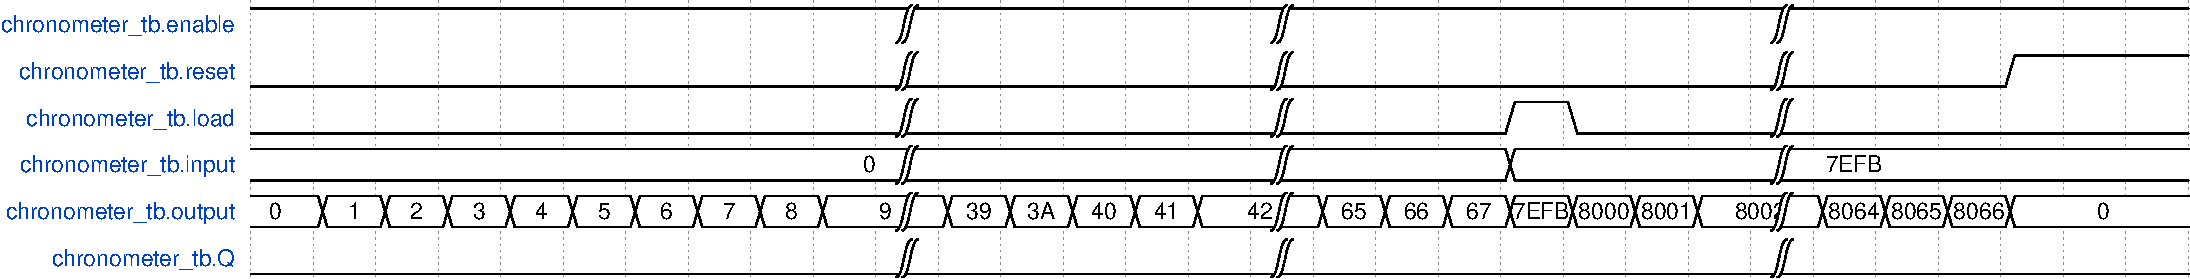
\includegraphics[width=\textwidth]{img/chronometer_tb.pdf}
    \caption{Simulazione del cronometro}
    \label{fig:chronometer_tb}
\end{figure}

\subsection{Esercizio 5.2}
Si implementa un cronometro su FPGA, con la visualizzazione del tempo su un display a sette segmenti e la possibilità di impostare manualmente il valore iniziale tramite switch e pulsanti.

\begin{code}
    \inputminted{vhdl}{vhdl/chronometer_onboard.vhd}
    \caption{Implementazione del cronometro su board}
    \label{cod:chronometer_onboard}
\end{code}

\begin{code}
    \inputminted{vhdl}{vhdl/chronometer_seven_segments_display.vhd}
    \caption{Implementazione del display a sette segmenti}
    \label{cod:chronometer_seven_segments_display}
\end{code}

\begin{code}
    \inputminted{vhdl}{vhdl/chronometer_cathodes_manager.vhd}
    \caption{Implementazione del gestore dei catodi}
    \label{cod:chronometer_cathodes_manager}
\end{code}

\begin{code}
    \inputminted{vhdl}{vhdl/chronometer_cathodes_input_manager.vhd}
    \caption{Implementazione del gestore input-catodi}
    \label{cod:chronometer_cathodes_input_manager}
\end{code}

\begin{code}
    \inputminted{vhdl}{vhdl/chronometer_input_manager.vhd}
    \caption{Implementazione del gestore degli input}
    \label{cod:chronometer_input_manager}
\end{code}

\paragraph{Funzionamento generale.}
Il cronometro conta il tempo nel formato HH:MM:SS e supporta un intervallo di [00:00:00; 23:59:59]. Quando raggiunge 23:59:59, riparte da 00:00:00 automaticamente. Per impostare manualmente il tempo di partenza vengono utilizzati gli switch e i pulsanti:

\begin{itemize}
    \item Switch: per inserire il valore desiderato in notazione binaria posizionale.
    \item \texttt{BTNR} (pulsante di destra): memorizza i secondi.
    \item \texttt{BTNC} (pulsante al centro): memorizza i minuti.
    \item \texttt{BTNL} (pulsante di sinistra): memorizza le ore.
    \item \texttt{BTND} (pulsante in basso): visualizza il valore memorizzato.
    \item \texttt{BTNU} (pulsante in alto): reset del cronometro.
\end{itemize}

Se un valore non valido (es. 63 secondi) viene inserito, il sistema lo azzera automaticamente.

\paragraph{Struttura del codice.}
L'architettura è strutturale, ovvero il sistema è composto da diversi moduli interconnessi:

\begin{enumerate}
    \item \texttt{chronometer\_onboard} [Codice sorgente \ref{cod:chronometer_onboard}]: modulo principale che definisce le interfacce tra il cronometro, i pulsanti, i display e il sistema di input.
    \item \texttt{chronometer} [Codice sorgente \ref{cod:chronometer}]: si occupa del conteggio del tempo basandosi su un segnale di clock e può essere impostato manualmente.
    \begin{itemize}
        \item Il cronometro utilizza un clock divider per generare un segnale di 1 Hz, così che i secondi avanzino correttamente.
        \item Se viene premuto \texttt{BTND}, viene caricato il valore impostato tramite \texttt{input\_time}.
        \item Se viene premuto \texttt{BTNU}, il cronometro si resetta.
    \end{itemize}
    \item \texttt{seven\_segments\_display} [Codici sorgente \ref{cod:chronometer_seven_segments_display}, \ref{cod:chronometer_cathodes_manager}, \ref{cod:chronometer_cathodes_input_manager}, \ref{cod:anodes_manager}]: mostra il tempo nel formato HH:MM:SS sul display a sette segmenti.
    \begin{itemize}
        \item Viene utilizzato uno scanning circuit per gestire le 6 cifre del display.
        \begin{itemize}
            \item Si utilizza uno scanning circuit in quanto il display a sette segmenti è dotato di 8 anodi (uno per cifra, ognuno in comune per tutti i segmenti della stessa) ed 8 catodi (uno per segmento, ognuno in comune per i segmenti analoghi di tutte le cifre). Di conseguenza è possibile attivare una sola configurazione dei segmenti alla volta. Il circuito funziona accendendo una cifra alla volta, ma a una velocità così alta che l'occhio umano non percepisce lo spegnimento, ed assegnando ogni volta una configurazione dei segmenti differente ad ogni cifra. Questo è ottenuto attivando ogni cifra in sequenza rapida (di solito 500 Hz o più), illuminandola per un breve periodo di tempo prima di passare alla successiva e creando l’illusione visiva che tutte le cifre siano accese contemporaneamente.
        \end{itemize}
        \item Il valore letto dal cronometro viene convertito nel formato corretto per il display.
    \end{itemize}
    \item \texttt{input\_manager} [Codice sorgente \ref{cod:chronometer_input_manager}]: gestisce gli input da switch e pulsanti, permettendo di impostare il tempo iniziale.
    \begin{itemize}
        \item Quando si preme \texttt{BTNL}, \texttt{BTNC} o \texttt{BTNR}, il valore attuale degli switch viene memorizzato come ore, minuti o secondi.
        \item Se il valore è fuori range, viene automaticamente azzerato.
    \end{itemize}
\end{enumerate}

Per poter utilizzare la board è stato necessario effettuare alcune modifiche al file dei constraints \texttt{Nexys A7-100T-Master.xdc}. In particolare, abbiamo dovuto aggiungere i seguenti vincoli:
\begin{itemize}
    \item Abilitare il clock a 100 MHz.
    \item Abilitare gli switch \texttt{SW0}--\texttt{SW5} per l’input.
    \item Abilitare i pulsanti \texttt{BTNL}, \texttt{BTNR} e \texttt{BTND} per il controllo del caricamento dei dati, \texttt{BTNU} per il reset.
    \item Abilitare i catodi \texttt{CATHODES0}--\texttt{CATHODES7} e gli anodi \texttt{ANODES0}--\texttt{ANODES7} per l'utilizzo del display a sette segmenti.
\end{itemize}
